%نام و نام خانوادگی:
%شماره دانشجویی: 
\مسئله{}
در متدولوژی \lr{Scrum}:
\\
الف) برای هر آیتم \lr{Product Backlog} فاکتوری به نام \lr{Estimate} یا تخمین وجود دارد. \\
چرا تخمین می‌تواند مهم باشد؟\\
پنج روش تخمین را تحقیق و به زبان خود در یک پاراگراف 4 یا 5 خطی توضیح دهید.\\
ب) یکی از مسئولیت‌های \lr{Product Owner} اولویت‌بندی آیتم‌های \lr{Product Backlog} است. پنج مورد از روش‌های اولویت‌بندی را تحقیق نموده و هر یک را به زبان خود در یک پاراگراف حداقل 5 خطی توضیح دهید.

\پاسخ{
	
الف) 
تخمین برای هر آیتم بک‌لاگ محصول از چند جهت می‌تواند مورد اهمیت باشد.

نخست، با استفاده از تخمین می‌توان اولویت کارها را مشخص کرد.
\lr{Product Owner}
از تخمین‌های انجام شده، می‌تواند دید کلی نسبت به میزان پیچیدگی هر آیتم به دست آورده و با توجه به این ویژگی در کنار ویژگی‌های دیگر هر آیتم، آن‌ها را اولویت‌بندی کند. هم‌چنین تخمین به \lr{Product Owner} کمک می‌کند که بتواند برنامه‌ریزی بهتری برای کارهای آینده‌ی پروژه انجام دهد. به طور مثال تصمیم بگیرد که بهترین انتخاب‌ها برای قرار گرفتن در لیست کارهای اسپرینت آینده کدام یک از آیتم‌ها هستند.

علاوه بر آن تخمین این امکان را به تیم می‌دهد که دیدی تقریبی از زمانی که می‌توانند هر قابلیت (\lr{Feature}) را ارائه دهند داشته باشد. معمولا افرادی که در سمت کسب‌و‌کار هستند نیاز به داشتن یک تخمین از آماده شدن یک محصول یا فیچر دارند و به همین علت نیاز است تیم امکان پاسخ‌گویی به این سوالات را داشته باشد. هر چه‌قدر تیم بتواند تخمین‌های بهتری بزند، ذی‌نفعان اعتماد بیشتری به تخمین‌های تیم خواهند کرد و می‌توانند با استفاده از آن‌ها تصمیمات بهتری برای کسب‌وکار بگیرند. این مسئله باعث افزایش اعتبار تیم نیز می‌شود.

اهمیت دیگر تخمین این است که این تضمین را می‌دهد که تسک‌ها تا حد ممکن برای اعضای تیم شفاف شده باشند. زیرا برای این که اعضا بخواهند به یک تسک تخمین بدهند لازم است به آن فکر کرده باشند و در صورت نیاز درباره‌ی آن صحبت نیز بکنند. در نتیجه در صورتی که نقاط مبهمی درباره‌ی وظایف وجود داشته باشد، متوجه آن خواهند شد و می‌توانند با گفت‌وگو بین اعضای تیم تا حد امکان این ابهامات را برطرف کنند. علاوه بر شفاف شدن آیتم‌ها، این کار باعث می‌شود تا همه‌ی اعضای تیم درک یکسانی از آیتم‌های مختلف پیدا کنند.


در ادامه، پنج روش پراستفاده‌ برای تخمین آورده شده است:

\begin{itemize}
\item
\lr{Planning Poker}:
در این روش لازم است ابتدا یک مقیاس برای تخمین زدن هر آیتم انتخاب شود. مقیاسی که معمولا مورد استفاده قرار می‌گیرد چند جمله‌ی اول دنباله‌ی فیبوناچی است؛ اما بسته به صلاح‌دید تیم می‌توان از دنباله‌ی دیگری از اعداد هم استفاده کرد. پس از انتخاب مقیاس مقداردهی، به هر کدام از اعضای تیم تعدادی کارت داده می‌شود که اعداد انتخاب شده  روی آن نوشته شده است. حال به اعضای هر آیتم در بک‌لاگ محصول، هر کدام از اعضای تیم از بین کارت‌هایی که دارند یکی را به عنوان تخمین خود برای آن آیتم انتخاب می‌کنند. لازم است تا قبل از این که همه‌ی اعضا تخمین خود را انتخاب کنند، هر کس مقدار کارت خود را مخفی نگه دارد تا هر عضو تیم نظر خودش را بدون تحت‌تاثیر قرار گرفتن توسط نظر افراد دیگر بدهد. پس از این که همه کارت خود را انتخاب کردند کارت‌ها دیده می‌شود و افرادی که کم‌ترین و بیش‌ترین مقدار تخمین را زده‌اند، علت انتخاب خود را می‌گویند. پس از آن دوباره هر کس با توجه به دید جدیدی که از صحبت‌ها به دست آورده تخمین خود را انتخاب می‌کند. زمانی که همه روی یک مقدار توافق کنند، آن مقدار (یا اگر تخمین‌ها خیلی نزدیک به هم باشد، میانگین آن‌ها) به عنوان تخمین نهایی آن آیتم در نظر گرفته می‌شود.

\item
\lr{T-shirt Sizing}:
در این روش از اندازه‌های معمول تیشرت، یعنی
\lr{XS}، \lr{S}، \lr{M}، \lr{L} و \lr{XL}
برای تخمین
\lr{Story Points}
هر آیتم استفاده می‌شود. پس از این که \lr{Facilator} یک آیتم را توضیح داد، در صورت نیاز صحبت‌هایی درباره‌ی آن آیتم و محدودیت‌ها و حوزه‌ی \lr{Scope} آن بین اعضای تیم صورت می‌گیرد. پس از آن هر فرد نظر خود را درباره‌ی این که کدام اندازه‌ی تیشرت بیشتر برای آیتم مناسب است ارائه می‌دهد و لازم است تا زمان رسیدن به توافق سر یک اندازه، اعضا با یک دیگر بحث کرده و علت انتخاب خود را توضیح دهند.

\item
\lr{The Bucket System}:
در این روش نیز لازم است ابتدا یک مقیاس نسبی برای تخمین‌دهی استفاده شود. پس از انتخاب آن، هر عدد روی یک کارت نوشته می‌شود. هر کدام از کارت‌ها نماینده‌ی هر کدام از سطل‌ها (\lr{Bucket}) هستند. در ابتدا یک آیتم بک‌لاگ محصول انتخاب شده و در سطل وسط قرار داده می‌شود. سپس باقی آیتم‌ها بین اعضای تیم پخش شده و هر کدام از اعضا با توجه به اندازه‌ی نسبی آیتم‌ها نسبت به کارت اولیه، اقدام به قرار دادن آیتم‌ها در سطل‌ها می‌کنند. در این گام نیازی به صحبت با بقیه اعضای تیم وجود ندارد و در صورتی که یکی از اعضا آیتمی را در اختیار داشته باشد که درباره‌ی آن اطلاعات کافی نداشته باشد، می‌تواند آن را به عضو دیگری از گروه بدهد. پس از اتمام این کار همه‌ی اعضا لیست کارهای داخل سطل‌ها را نگاه می‌کنند و در صورتی که از نظرشان آیتمی در جای مناسب قرار نگرفته بود، آن را مطرح کرده و با بحث بین اعضای گروه به توافق برای جایگاه درست آن آیتم می‌رسند. 

\item
\lr{Three-Point Estimate}:
در این روش، ابتدا برای هر آیتم بک‌لاگ سه مقدار تخمین زده می‌شود: اندازه در بهترین‌ حالت، اندازه در بدترین حالت، اندازه در حالت معمول یا حالتی که بیشترین احتمال رخ دادن را دارد. پس از آن با استفاده از میانگین عادی یا میانگین وزن‌دار این سه مقدار (معمولا با وزن‌دهی بیشتر به مقدار سوم) یک تخمین نهایی برای هر تسک داده می‌شود. یکی از مزیت‌های این روش این است که لازم می‌شود اعضای تیم در هنگام تخمین به مشکلات احتمالی فکر کنند و در صورت امکان در جهت پیش‌گیری از آن‌ها کارهایی انجام دهند.

\item
\lr{Ordering Protocol}:
در این روش، هدف این است که آیتم‌ها را به ترتیب اندازه‌ی تخمینی نسبت به هم در یک ردیف قرار داده شوند. برای این کار می‌توان از یک میز استفاده کرد که یک سر آن بزرگ‌ترین آیتم‌ها‌ و سر دیگر آن کوچک‌ترین آیتم‌ها قرار می‌گیرند. در صورت نیاز می‌توان یک مقیاس هم روی میز برای داشتن یک دید اولیه قرار داد. در هر گام، اعضای تیم یک آیتم را برداشته و با توجه به تخمین خود در یک نقطه روی میز قرار می‌دهند. با توجه به اندازه‌ی آیتم‌ها نسبت به یک‌دیگر، می‌توان تصمیم گرفت که یک آیتم در کدام سمت آیتم دیگر قرار بگیرد. هم‌چنین می‌توان کارت‌هایی که پیش از این روی میز قرار داده شده‌اند را هم جابه‌جا کرد تا ترتیب بهتری به دست آید.


\end{itemize}


ب)
\begin{itemize}
    \item مسیر بحرانی

    وقتی تیم‌ها به تازگی با روش جابک شروع به کار می‌کنند یا مثلا در حال اجرای روشی هیبریدی هستند، اغلب برای برخی مسائل ضرب‌الاجل دارند. برای رسیدن به این اهداف، یوزر استوری‌های مشخصی وجود دارد در روندی آبشاری به هم وابسته‌اند و باید تکمیل شوند. به این مسیر از وظایف، مسیر بحرانی می‌گوییم و مجموع زمانی که برای اتمام می‌گیرند، حداقل زمان برای اجرای کارهاست. اگر تیم در وضعیتی باشد که اهدافی با ضرب‌العجل‌های مشخص دارد اجرای تکنیک مسیر بحرانی می‌تواند کارهای مهمی که باید انجام شوند تا راه برای کار‌های دیگر باز شود را پیدا کند.
    \item رتبه‌بندی پشته‌ای

    رتبه‌بندی پشته‌ای با مرتب‌سازی هر کار بر اساس اولویت انجام می‌شود. به این ترتیب، کارهای با بالاترین اولویت در بالاترین رتبه و به دنبال آن کارهای مهم بعدی به ترتیب قرار میگیرند. وقتی با یک بک‌لاگ بزرگ و نامرتب مواجه می‌شوید، اینکه متوجه شویم کار شماره‌ی ۱۰ در جای مناسبی قرار دارد یا نه کار سخت‌تری از بررسی اینکه کار شماره‌ی ۱۰ باید بالاتر یا پایین‌تر از کار شماره‌ی ۱۱ باشد، است. به این فرایند مقایسه هر مورد با تنها یک مورد دیگر و تصمیم‌گیری اینکه کدام یک اولویت بالاتر است، رتبه‌بندی پشته‌ای می‌گوییم.

    \item کار‌های با کمترین زحمت، اول!
    
    این اولویت‌بندی بر انجام کارهایی متمرکز است که کمترین میزان کار را می‌طلبد. این کار در اسکوپ گروهی ممکن است زمان و انرژی زیادی ببرد زیرا باید کارها بر اساس زحمتی که می‌برند مرتب شوند تا کم‌زحمت‌ترین کار انتخاب شود. در موارد زیر بهره‌بری از این تکنیک مناسب است:
    \begin{itemize}
        \item زمان کوتاهی برای انجام کاری در اختیار دارید.
        \item می‌خواهید افراد تیم را به حرکت‌کردن وادار کنید. برخی تیم‌ها دچار سستی و کرختی می‌شوند در این شرایط با انجام کارهایی که هم کم‌زحمت هستند و هم به سرعت تمام می‌شوند احساس خوب پیشرفت را به تیم هدیه می‌دهید.
        \item اگر تعداد زیادی باگ ریز دارید که به سرعت می‌توان تصحیحشان کرد.
    \end{itemize}
    توجه داشته باشید که این تکنیک اصلا به ارزش کاری که انجام می‌دهید اهمیت نمی‌دهد و ممکن است کارهای مهم و باارزش را برای مدتی طولانی عقب بیاندازید زیرا هرگز کم‌زحمت نبودند!

    \item روش \lr{CD3}
    
    روش هزینه تاخیر یک روش بسیار تاثیر گذار برای اولویت‌بندی بک‌لاگ است که می‌تواند خطر زیان احتمالی را کاهش دهد. صاحب محصول، مورد‌های با بالاترین هزینه را ارزیابی کرده و آن‌ها را در بالای لیست بک‌لاگ قرار می‌دهد. همچنین کارهایی که امکان تحمل نمودن بیشترین ضرر به شرکت را دارند ارجحیت دارند. در واقع در این روش تصمیم می‌گیرید برخی کارها به زمانی دیگر موکول شوند تا جا برای کارهای مهم‌تر باز شود. روش هزینه تأخیر چالشی است زیرا مانند قسمت قبل هزینه هر یک از آیتم های بک‌لاگ باید بررسی شود و این فرآیند را پیچیده و طولانی می‌کند. مثلا زمانی که باید یک محصول پیش از یک تاریخ خاص فصلی (مانند جمعه‌ی سیاه) روانه‌ی بازار شود باید در اولویت کارها تجدید نظر کرد.
    
 \begin{figure}[h]
   	\centering
   	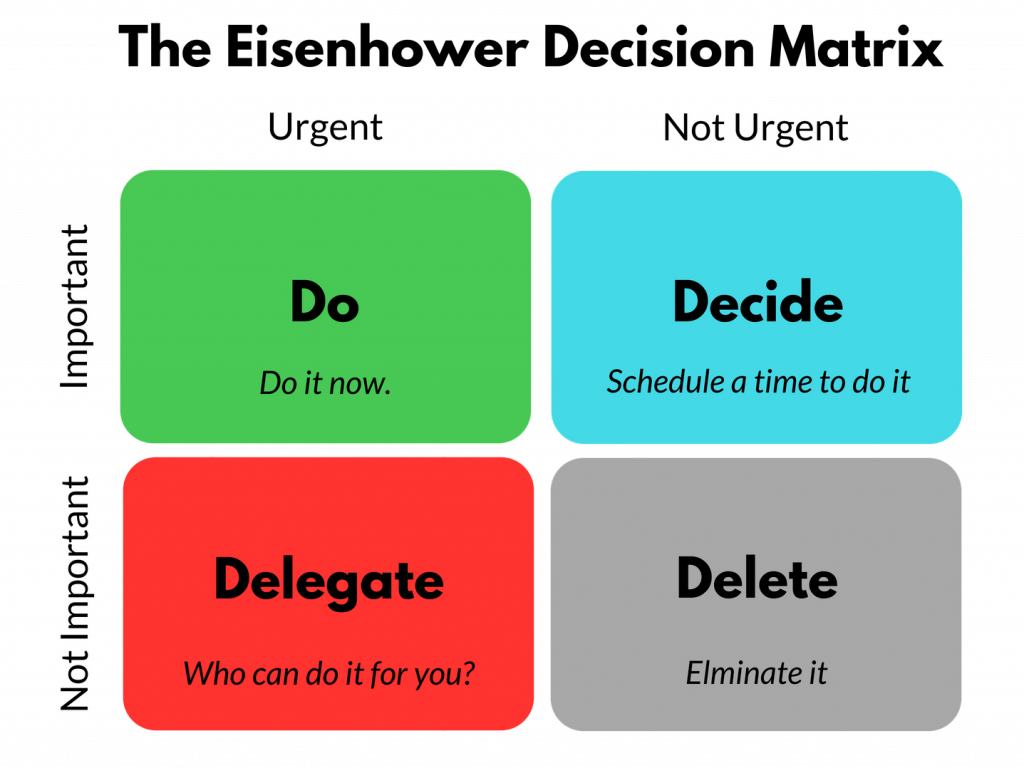
\includegraphics[scale=0.3]{figs/3-2}
   	\caption{ماتریس آیزنهاور}
\end{figure}

    \item ماتریس آیزنهاور

 این ماتریس به احترام رئیس‌جمهور اسبق آمریکا آیزنهاور نامیده شده. این یک روش برای اولویت‌بندی کار هاست که نه تنها در کارهای تیمی، که در زندگی روزمره بسیار مفید است. در این روش کار‌ها از دو منظر بررسی می‌شوند؛ اهمیت و اضطرار. بنابراین هر کار در یکی از چهاردسته می‌افتد: مهم و ضروری، مهم ولی غیرضروری، کم‌اهمیت ولی ضروری و کم‌اهمیت و غیرضروری. با کار‌های درون هر کدام از این ۴ خانه باید یک کار مشخص انجام داد.
    \begin{itemize}
        \item مهم و ضروری: اکنون انجامش بده!
        \item مهم ولی غیر ضروری: زمانی را برای انجام آن تعیین کن.
        \item کم‌اهمیت ولی ضروری: انجام این کار را به کسی دیگر محول کنید.
        \item کم‌اهمیت و غیر ضروری: این کار را فعلا حذف کنید.
    \end{itemize}
    به این صورت می‌توان بک‌لاگ را در تیم اولویت‌بندی کرد تا نظم بر کارها حاکم شود.
\end{itemize}

}

\subsection*{مراجع}

\begin{latin}
	\begingroup
	\renewcommand{\section}[2]{}%
	
	\begin{thebibliography}{9}
		%   https://www.student.unsw.edu.au/how-do-i-cite-electronic-sources
		
		\bibitem{3-1-2}
		Slava Moskalenko,
		2017,
		\textit{Scrum.org},
		What Scrum Says About Estimates, 
		accessed 8 November 2022,
		\url{https://www.scrum.org/resources/blog/what-scrum-says-about-estimates}
		
		
		\bibitem{3-1-1}
		Mike Cohn,
		2022,
		\textit{Mountain Goat Software},
		Four Reasons Agile Teams Estimate Product Backlog Items, 
		accessed 8 November 2022,
		\url{https://www.mountaingoatsoftware.com/blog/four-reasons-agile-teams-estimate-product-backlog-items}
		
		\bibitem{3-1-3}
		Krzysztof Sowa,
		2019,
		\textit{Concise Software},
		How to estimate product backlog effectively, 
		accessed 8 November 2022,
		\url{https://medium.com/@concisesoftware/how-to-estimate-product-backlog-effectively-aefa4b9051aa}
		
		\bibitem{3-1-4}
		Deepti Sinha,
		2022,
		\textit{Knowledgehut},
		Top 5 Scrum Estimation Techniques- Find Your Best Fit, 
		accessed 8 November 2022,
		\url{https://www.knowledgehut.com/blog/agile/top-5-scrum-estimation-techniques-find-your-best-fit}
		
		\bibitem{3-1-5}
		Vibhuti Verma,
		2021,
		How to estimate an Agile Backlog?,
		accessed 8 November 2022,
		\url{	https://www.linkedin.com/pulse/how-estimate-agile-backlog-vibhuti-verma}

		\bibitem{3-1-6}
		\textit{TutorialsCampus},
		Estimation Techniques,
		accessed 9 November 2022,
		\url{	https://www.tutorialscampus.com/agile/estimation-techniques.htm}
		
		\bibitem{3-1-7}
		\textit{wrike},
		How Does a Product Owner Prioritize Backlog,
		accessed 9 November 2022,
		\url{	https://www.wrike.com/product-management-guide/faq/how-does-a-product-owner-prioritize-backlog/}

		\bibitem{3-1-8}
		\textit{parabol},
		How to Prioritize the Backlog When Everything is Important,
		accessed 9 November 2022,
		\url{	https://www.parabol.co/blog/product-backlog-prioritization-techniques/}

		\bibitem{3-1-8}
		\textit{LUXAFOR},
		The Eisenhower Matrix: Time and Task Management Made Simple,
		accessed 9 November 2022,
		\url{	https://luxafor.com/the-eisenhower-matrix/}
	
	\end{thebibliography}
	\endgroup
\end{latin}